%%%%%%%%%%%%%%%%%%%%%%%%%%%%%%%%%%%%%%%%%%%%%%%%%%%%%%%%%%%%%%%%%%%%%%%%%%%%%%%
%
% Tommy P. Keane
% Master of Science Thesis
% Department of Electrical and Microelectronic Engineering
% Rochester Institute of Technology
%
% April 2011
%
%
%
% Funded By: Lenel Systems Inc., A UTC Fire & Security Corporation
%
% Algorithm Intellectual Property Owned By: Lenel Systems Inc.
%
%
% http://www.tommypkeane.com
%
%%%%%%%%%%%%%%%%%%%%%%%%%%%%%%%%%%%%%%%%%%%%%%%%%%%%%%%%%%%%%%%%%%%%%%%%%%%%%%%

%%%%%%%%%%%%%%%%%%%%%%%%%%%%%%%%%%%%%%%%%%%%%%%%%%%%%%%%%%%%%%%%%%%%%%%%%%%%%%%
%
% CHAPTER 3
%
% SECTION 1: Algorithm Components
%
%%%%%%%%%%%%%%%%%%%%%%%%%%%%%%%%%%%%%%%%%%%%%%%%%%%%%%%%%%%%%%%%%%%%%%%%%%%%%%%


%%%%%%%%%%%%%%%%%%%%%%%%%%%%%%%%%%%%%%%%%%%%%%%%%%%%%%%%%%%%%%%%%%%%%%%%%%%%%%%
% BEGIN DOCUMENT

The basic algorithm contains 5 major steps as shown in the flowchart in Figure \ref{algorithmFlowchart} below. This chart shows the processing order of each step, but purposefully has labeled them by their goal and not their specific implementation details. The exact processes of the algorithm will be explained in the following subsections, but, as is the intended purpose of the flowchart, it should be kept in mind that the specific operations were chosen to serve the goals. The overall algorithm itself could be implemented differently as long as the main goals in each step are met. This will be discussed further in Chapter 6 as a possibility for future work in modifying some of the chosen means of implementing these components. The development of the implementation is presented in Chapter 4, but for now each component will have its purpose and method of implementation presented.

\begin{figure}
\label{algorithmFlowchart}
\centering
\vskip-.25in
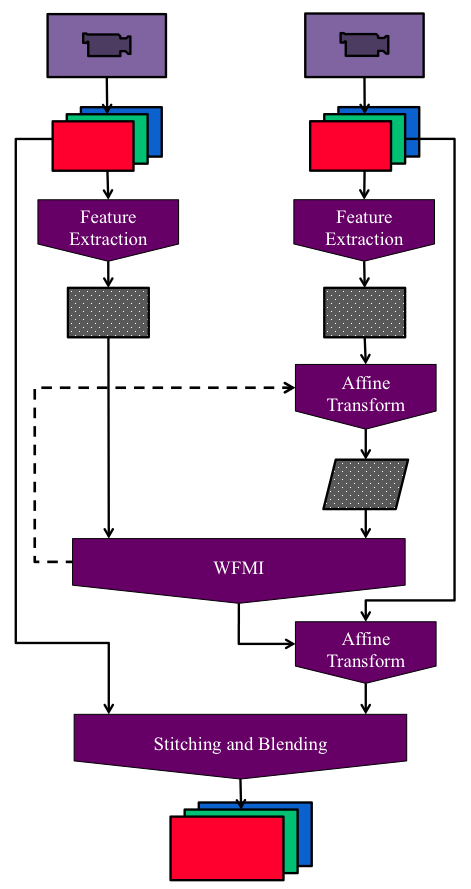
\includegraphics[height=1\textheight]{algorithmFlowchart}
\caption{Flowchart}
\end{figure}


%%%%%%%%%%%%%%%%%%%%%%%%%%%%%%%%%%%%%%%%%%%%%%%%%%%%%%%%%%%%%%%%%%%%%%%%%%%%%%%
% END OF DOCUMENT
